\documentclass[12pt]{article}
\usepackage[utf8]{inputenc}
\usepackage[russian]{babel}
\usepackage{graphicx}
\usepackage{algpseudocode}
\usepackage{algorithm}
\usepackage{algorithmicx}
\usepackage{tikz}
\usepackage{pgfplots}
\usepackage{url}

\usetikzlibrary[decorations.shapes]

\pgfplotsset{width=7cm}

\renewcommand{\labelenumi}{\arabic{enumi})}

\author{Чуприков Павел Сегреевич \\ группа 4539\\}
\title{Отчет по курсовой работе по теме: <<Расчет дискретной временной диаграммы 
Вороного с применением графического процессора>>}
\begin{document}

\begin{titlepage}
\thispagestyle{empty}
\begin{center}
Санкт-Петербургский 
национальный исследовательский университет информационных технологий,
механики и оптики\\
\smallskip
Факультет информационных технологий и программирования\\
\smallskip
Кафедра компьютерных технологий\\
\vspace{2cm}
\large{Чуприков Павел Сергеевич}\\
\vspace{1cm}
\begin{LARGE}
Отчет о курсовой работе по теме: <<Расчет дискретной временной диаграммы 
Вороного с применением графического процессора>>\\
\end{LARGE}
\vfill
\today
\end{center}
\end{titlepage}
\setcounter{page}{2}
\tableofcontents

\pagebreak

\section{Введение}
\emph{Диаграмма Вороного} --- широко известный и глубоко изученный предмет
вычислительной геометрии. Ее можно кратко описать как способ разбиения
плоскости, в котором сначала выделяется некоторое множество точек-источников
(здесь и далее элементы этого и подобных множеств будем называть \emph{источниками},
англ. --- seed), и затем любая другая точка плоскости <<красится>> в цвет ближайшей к ней 
(относительно какой-то заданной метрики) точки-источника. 
Диаграммы имеют множество применений в таких
задачах, как определение столкновений при физических расчетах, 
планирование маршрута, кластеризация данных. Более подробный обзор 
можно найти в работе \cite{survey}. Также нашли применение и визуальные качества такого
разбиения плоскости: например, в области процедурной генерации текстур \cite{proced} (рис.~\ref{rocks}). 

\begin{figure}
\begin{center}
\includegraphics[scale=1]{voronoi_rocks.png}
\end{center}
\caption{Текстура, основанная на диаграмме Вороного, сгенерированная процедурно.}
\label{rocks}
\end{figure}

Более информативным расширением диаграмм Вороного является \emph{преобразование 
расстояний} (поле расстояний, карта расстояний), сопоставляющее каждой точке 
пространства расстояние до некоторого объекта (источника). Области применения 
поля расстояний включают: определение столкновений, навигацию объектов 
искусственного интеллекта, отрисовка векторных данных.

И первая, и вторая геометрические конструкции легко обобщаются на случай, когда 
в качестве источников выступают не точки, а отрезки, окружности или любые другие
геометрические фигуры.

Нужно отметить, что и диаграмма Вороного, и поле расстояний --- это 
математические объекты, для практического их применения в программных 
продуктах существует два принципиально различных метода хранения этих
объектов (точнее, их приближений) --- \emph{векторный} и \emph{дискретный}.
Можно привести аналогию с векторным и растровым способами представления 
изображений в памяти компьютера соответственно. В первом случае 
диаграмма Вороного хранится в виде некоторой структуры данных, например 
\emph{двусвязный список ребер} (англ. Double Connected Edge List --- DCEL),
во втором случае --- область, для которой строится диаграмма Вороного, 
дискретизируется тем или иным образом, и для каждого узла дискретизации хранится
цвет или расстояние.

Несмотря на то, что существует множество алгоритмов разной степени 
эффективности для построения как диаграмм Вороного, так и поля расстояний,
в них обычно используется стандартная Евклидова метрика. Однако, часто одного
расстояния недостаточно, может потребоваться фактическое время, которое 
необходимо затратить для перемещения из точки-источника в какую-либо точку
плоскости. Расчет времени требует знания скорости перемещения, а скорость не всегда постоянна
в области, поэтому стандартная Евклидова метрика в данном случае не годится.
В статье \cite{timeb} описывается построение временной 
диаграммы Вороного в присутствии двух бесконечных прямых, скорость перемещении
вдоль которых не совпадает со скоростью в остальной части плоскости.

Простейший пример неоднородности можно найти в задачах планирования маршрута
на местности, для которой характерно наличие различных по проходимости участков,
а главное --- быстро проходимых дорог. В данной работе описывается метод, 
который при некоторых (весьма строгих) упрощениях позволяет построить 
поле расстояний или диаграмму Вороного, основанные на времени,
для дискретного случая их представления.

\section{Постановка задачи}
\label{task}
Итак, далее рассматривается построение т.~н. \emph{временной диаграммы Вороного}
(англ. Time-based Voronoi diagram) некоторой области, которая будет 
вычисляться не по расстоянию, а по времени, для этого на всей области
необходимо определить некоторое поле скоростей.

\subsection{Условия, входные и выходные данные}
\label{props}

\paragraph{Условие задачи.} Ниже перечислены
основные условия и свойства задачи, решение которой представлено в данной работе:
\begin{itemize}
\item \textbf{область построения диаграммы Вороного} --- прямоугольник, 
скорость в котором постоянна (будем называть данную скорость \emph{внешней}), за 
исключением некоторых \emph{областей неоднородности} (см. далее);
\item \textbf{структура представления} --- дискретная, прямоугольник разбивается на 
ячейки равномерной сеткой;
\item \textbf{форма источников} --- отрезки (точки как вырожденный случай)
на плоскости, для вершины $v$ отрезка должно быть указано время $T_{out}(v)$, 
которое необходимо  затратить, 
чтобы в нее попасть (внешняя информация от вышележащей структуры);
\item \textbf{области неоднородности} --- это сами источники, 
при этом скорость вдоль каждого отрезка может отличатся от
внешней скорости;
\item \textbf{структура пути}: считается, что маршрут, начинаясь в источнике,
некоторое время движется вдоль соответствующей области неоднородности.
Если он ее покидает, то далее скорость совпадает с внешней.
\end{itemize}

\paragraph{Выходные данные.}
Выходом работы алгоритма станет <<раскраска>> области, 
а именно --- каждой ячейки сетки $c$ будет сопоставлен такой источник, 
что для какой-либо вершины $v$ источника сумма $T_{out}(v)$ и времени от 
$v$ до $c$ (обозначение: $T(v, c)$) минимальна.

\subsection{Постоянство внешней скорости}
\label{multi_type}
Это ограничение достаточно серьезно, так как оно расходится с 
реальностью: проходимость в лесу может существенно отличаться от проходимости 
в поле или в болоте. 

Пусть область можно разбить на несколько выпуклых подобластей, скорость внутри которых
постоянна. В таком случае предлагается достаточно простой способ вычислить временную
диаграмму Вороного, при фиксированном ограничении на число переходов между областями.
Способ схож с алгоритмом Форда-Беллмана ~\cite{cormen} нахождения 
кратчайшего пути во взвешенном графе от заданной вершины до всех остальных. 
Если предположить, что запуск алгоритма вычисления временной диаграммы Вороного 
внутри подобласти --- это своего рода релаксация ребер внутри подобласти, 
а источники вместе с границами областей
--- это вершины, то каждый путь от источника до вершины можно представить
как некоторый путь в таком графе. 

Ниже приведено описание алгоритма для случая, когда пересекать границу разрешается 
не более одного раза
(рис.~\ref{multi_type_fig}):
\begin{enumerate}
\label{multi_type_algo}
\item для каждой подобласти вычислить диаграмму Вороного отдельно, используя
скорость внутри выбранной подобласти;
\item добавить к точкам-источникам каждой подобласти ее границу, используя посчитанное в
предыдущем шаге время от источников до точек границы;
\item  вычислить диаграммы внутри подобластей, используя новые точки-источники.
\end{enumerate}
\begin{figure}
\begin{center}
\begin{tikzpicture}[scale=5]
\coordinate (a) at (0, 0);
\coordinate (b) at (1, 0);
\coordinate (c) at (1, 1);
\coordinate (d) at (0, 1);
\coordinate (ab) at (0.3, 0);
\coordinate (bc) at (1, 0.7);
\coordinate (cd) at (0.4, 1);
\coordinate (da) at (0, 0.8);
\coordinate (center) at (0.6, 0.5);
\path[fill, red!40] (a) -- (ab) -- (center) -- (da);
\path[fill, green!40] (b) -- (bc) -- (center) -- (ab);
\path[fill, blue!40] (c) -- (cd) -- (center) -- (bc);
\path[fill, yellow!40] (d) -- (da) -- (center) -- (cd);
\begin{scope}[decoration={shape backgrounds, shape=rectangle, shape size = 2pt,
raise = 2pt, shape sep=4pt}]
\draw[decorate, red, fill] (ab) -- (center);
\draw[decorate, green, fill] (center) -- (ab);
\draw[decorate, green, fill] (bc) -- (center);
\draw[decorate, blue, fill] (center) -- (bc);
\draw[decorate, blue, fill] (cd) -- (center);
\draw[decorate, yellow, fill] (center) -- (cd);
\draw[decorate, yellow, fill] (da) -- (center);
\draw[decorate, red, fill] (center) -- (da);
\end{scope}
\draw (a) rectangle (c);

\coordinate (a') at (1.3, 0);
\coordinate (b') at (2.3, 0);
\coordinate (c') at (2.3, 1);
\coordinate (d') at (1.3, 1);
\coordinate (ab') at (1.6, 0);
\coordinate (bc') at (2.3, 0.7);
\coordinate (cd') at (1.7, 1);
\coordinate (da') at (1.3, 0.8);
\coordinate (center') at (1.9, 0.5);

\path[fill, red!40] (a') -- (ab') -- (center') -- (da');
\path[fill, green!40] (b') -- (bc') -- (center') -- (ab');
\path[fill, blue!40] (c') -- (cd') -- (center') -- (bc');
\path[fill, yellow!40] (d') -- (da') -- (center') -- (cd');
\begin{scope}[decoration={shape backgrounds, shape=rectangle, shape size = 2pt,
raise = 2pt, shape sep=4pt}]
\draw[decorate, green, fill] (ab') -- (center');
\draw[decorate, red, fill] (center') -- (ab');
\draw[decorate, blue, fill] (bc') -- (center');
\draw[decorate, green, fill] (center') -- (bc');
\draw[decorate, yellow, fill] (cd') -- (center');
\draw[decorate, blue, fill] (center') -- (cd');
\draw[decorate, red, fill] (da') -- (center');
\draw[decorate, yellow, fill] (center') -- (da');
\end{scope}
\draw (a') rectangle (c');
\draw[double = black, ->] (1.02, 0.5) -- (1.28, 0.5);
\end{tikzpicture}
\end{center}
\caption{Построение диаграммы с множеством различных подобластей. 
Слева --- запуск метода внутри подобластей
для получения информации о граничных точках, справа --- запуск метода
с новыми источниками (граничными точками).}
\label{multi_type_fig}
\end{figure}

\subsection{Области неоднородности}
Ограничения на области неоднородности, введенные ранее, предполагают следующее:
\begin{itemize}
\item существует некоторая внешняя реберная структура (например, граф дорог), 
которая допускает расчет кратчайших расстояний до каждого ребра, используя
только движение вдоль своих ребер.
\item движение вдоль ребер структуры быстро относительно внешней скорости 
настолько, что кратчайшему по времени маршруту хватает только однократного использования
ребер структуры.
\end{itemize}
Входные данные, подходящие под данное предположение, могут представлять
некоторую местность, возможно разнородную (см. предыдущий подраздел), на которой
расположена некоторая сеть дорог, скорость вдоль которых
значительно выше внешней скорости. Для каждой точки местности хотелось бы
узнать, за какое кратчайшее время и каким способ можно добраться 
из заданной точки до какого-либо из заданных пунктов, расположенных вдоль дорог.

Возможное решение описанной задачи может быть следующим:
\begin{enumerate}
\item решить задачу для графа дорог;
\item определить, используя данные предыдущего шага, для каждого ребра 
ближайший к нему пункт и соответствующее время;
\item отдать на вход методу, решающему задачу, поставленную в начале
данного раздела, информацию, полученную на предыдущем шаге,
и в итоге получить дискретизацию местности, каждая ячейка которой
<<знает>> ребро, ведущее к ближайшему пункту.
\end{enumerate}

Пример, изложенный выше, поясняет пункты условия задачи, изложенные ранее 
(см. подраздел ~\ref{props}).

\section{Обзор предыдущих методов}
\label{past}
В начале этой части будет рассмотрен метод, или, точнее, класс методов
вычисления дискретных диаграмм Вороного, который возможно разбить
на множество независимых потоков исполнения. Затем будет приведен
вариант обобщения метода для источников произвольной формы и, 
наконец, несколько простых результатов, полученные в работе \cite{timeb}, 
которые касаются, собственно, временных диаграмм Вороного.

\subsection{Jump-Flooding Algorithm (JFA)}
\label{jfa_desc}
Идеи рассматриваемого далее алгоритма впервые были представлены в работе
Дэниелсона \cite{distmap} в 1980~г. Однако, из-за отсутствия в то время
архитектуры, позволяющей одновременное выполнения большого числа потоков,
эти идеи тогда оказались неприменимы на практике. Спустя чуть более чем 20 лет, 
Гуодонг Ронг и Тиоу-Сенг Тан \cite{jfa} на основе работы Дэниелсона разработали 
алгоритм построения дискретной диаграммы Вороного, хорошо реализуемый
с помощью современных массивно-параллельных процессоров 
(англ.~massively-parallel processors), используемых в видеокартах и
специальных вычислительных сопроцессорах, таких как NVidia\textregistered \, 
Tesla\texttrademark.


Основу алгоритма составляет так называемый метод \textbf{JFA} (англ.
Jump-Flooding Algorithm). Опишем далее применение этого метода для 
построения диаграммы Вороного. 

Пусть на вход приходит дискретизация прямоугольной области 
равномерной сеткой размера $m \times n$. Каждая ячейка $\mathrm{cell}_{ij}$ 
содержащая точку-источник, хранит информацию $\mathrm{seed}_{ij}$ о его месте нахождения,
точки, не содержащие источник, хранят пустой идентификатор ${\mathrm{null}}$:
$$
	\mathrm{cell}_{ij} = \left\lbrace
	\begin{array}{ll}
	\mathrm{seed}_{ij}, & \mbox{в ячейке есть точка-источник;} \\
	\mathrm{null}, & \mbox{в ячейке нет точки-источника.}
	\end{array}
	\right.
$$

Далее информация об источниках распространяется на остальные ячейки
сетки, и в каждой ячейке будет содержаться информация 
о ближайшем источнике, про который данной ячейке известно на текущий момент. 
Распространение осуществляется в несколько итераций. Во время итерации 
каждая ячейка в отдельном потоке исполнения получает информацию об 
источниках от некоторых других ячеек, и таким образом пытается улучшить
собственную информацию об источнике. Пусть  $k = \max(\lfloor\log_2n\rfloor, \lfloor\log_2m\rfloor)$, 
тогда алгоритм выполнит $k$ итераций, при этом действия ячейки $\mathrm{cell}_{rc}$ 
в $i$-ую из них можно описать следующим образом:

\begin{algorithm}
\begin{algorithmic}
\State $\mathrm{mindist} \leftarrow \infty$
\State $\mathrm{step} \gets 2^{k - i}$
\State $p \gets r - \mathrm{step}$
\While{ $p \le r + \mathrm{step}$}
	\State $q \gets c - \mathrm{step}$
	\While{$q \le c + \mathrm{step}$}
		\If {$\mathrm{cell}_{pq} \neq \mathrm{null}$}
			\State $\mathrm{mindist} \gets 
 					\min(\mathrm{distanceTo}(\mathrm{cell}_{pq}), \mathrm{mindist})$
		\EndIf
		\State $q \gets q + \mathrm{step}$
 	\EndWhile
\State $p \gets p + \mathrm{step}$
\EndWhile
\end{algorithmic}
\caption{Поведение ячейки $\mathrm{cell}_{rc}$ во время $i$-ой итерации
\emph{JFA}}
\label{jfa_algo}
\end{algorithm}

Всего рабочую сложность (англ.~work complexity) алгоритма можно оценить 
как $O(m n k)$, при этом шаговая сложность (англ.~step complexity) --- $O(k)$. 
Для увеличения точности метода в статье предлагается выполнять 
еще одну итерацию с $\mathrm{step}~=~1$. Эксперименты подтверждают 
сокращение числа ошибок при данной модификации. Дальнейшее уменьшение числа 
ошибок с последующими итерациями незначительно. 
Модификацию \emph{JFA} с дополнительной итерацией обозначают как \emph{JFA+1}.

\paragraph{Реализация.} Авторами статьи метод был реализован с использованием 
графического процессора. Информация о ячейке хранилась в двумерной текстуре. 
На каждой итерации полноэкранный прямоугольник отрисовывался во внеэкранный
фреймбуффер (англ.~framebuffer). Каждой ячейке сетки соответствовал выходной
пиксель этого фреймбуффера и описанный в начале подраздела алгоритм
выполнялся на фрагментном шейдере.

\subsection{Обобщенные диаграммы Вороного, их вычисление с помощью графических 
процессоров}
\label{gvd}
В предыдущем методе в качестве источников рассматривались точки на плоскости, 
однако во введении мы упомянули о том, что источники можно обобщить. В статье 
2011 года \cite{gvd} Чжан Юан, Гуодонг Ронг и др. исследовали возможность
вычисления подобных обобщенных диаграмм Вороного (англ.~Generalized Voronoi
Diagram) с использованием графического  процессора. В работе рассматривались 
следующие возможные формы источников:

\begin{itemize}
\item точка;
\item отрезок;
\item окружность;
\item дуга окружности.
\end{itemize}

\paragraph{Ключевые идеи.} Опишем две ключевые идеи, использованные для
построения обобщенных диаграмм Вороного:
\begin{itemize}
\item Информация об источниках хранится отдельно от текстуры, представляющей
дискретизацию области. Вместо этого для хранения данной информации выделяется 
специальная одномерная текстура. В ячейках сетки хранится лишь индекс 
источника в этой одномерной текстуре источников.
\item Для того, чтобы внести информацию об источниках в равномерную сетку 
до первой итерации, применялись стандартные средства растеризации, реализованные 
в современных графических библиотеках.
\end{itemize}
Имея дискретизацию области с информацией об источниках далее остается
запустить изложенные ранее итерации алгоритма \emph{JFA} с модифицированным 
вычислением расстояния от ячейки до источника. Модификация заключается в том, что
необходимо вычислять расстояние не только от точки до точки, а также от точки до отрезка 
(окружности, дуги окружности). Тем не менее расстояние до источника любой
перечисленной формы можно вычислить за константное время, 
используя несложные геометрические соображения.

\paragraph{Замечание о памяти.} Заметим, что уменьшение шага дискретизации
в данном методе приводит к меньшим темпам роста объемов используемой памяти,
чем в предыдущем методе. В ячейке хранится 
лишь индекс, который обычно можно уместить в двухбайтовый целочисленный тип,
в то время как предыдущий метод хранил информацию о точке, что может
требовать вплоть до восьми байт (два числа с плавающей точкой одинарной точности).
Однако, суммарный объем информации, который необходимо считать из графической памяти,
оказывается больше, ведь кроме данных об источнике, которые
стали занимать больше места (четыре числа для отрезка), нужно еще 
сначала считывать индекс. Из-за особенностей подсистемы памяти,
которая объединяет запросы к последовательным кускам в отдельную 
транзакцию, производительность может пострадать еще больше, потому как 
доступ к одномерной текстуре с информацией об источниках в отличие от доступа
к ячейкам --- произвольный.

\paragraph{Результаты.} В работе \cite{gvd} было проведено сравнение с методом
$JFA$, полученные в результате графики представлены на рис.~\ref{fig_jfagvd}.
\begin{figure}
\begin{center}
\begin{tabular}{l l}
\begin{tikzpicture}
\begin{axis}[
    xtick = {1, 2, 3, 4},
    xticklabels={512, 1024, 2048, 4096},
    ylabel = {число ошибок, \%},
    xlabel = $n$ --- размер текстуры (текселей),
    ymax = 100,
    ytick = {0, 20, ..., 100},
    legend style={at={(0.5,1.1)},
        anchor=south,legend columns=3},
    ]
    \addplot+[sharp plot] coordinates
        {(1, 19) (2,7) (3,3.5) (4,2)};
    \addplot+[sharp plot] coordinates
        {(1, 2.7) (2,1) (3,0) (4,0)};
    \legend{JFA, GVD};
\end{axis}
\end{tikzpicture}
&
\begin{tikzpicture}
\begin{axis}[
    xtick = {1, 2, 3, 4},
    xticklabels={10, 100, 1000, 10000},
    ylabel = время работы (мс),
    xlabel = $n$ --- число отрезков,
    ymin = 0,
    legend style={at={(0.5,1.1)},
        anchor=south,legend columns=3},
    nodes near coords
    ]
    \addplot+[sharp plot] coordinates
        {(1, 22.34) (2, 22.54) (3, 22.78) (4,22.78)};
    \addplot+[sharp plot] coordinates
        {(1, 27.29) (2, 28.31) (3, 30.76) (4,31.14)};
    \legend{JFA, GVD};
\end{axis}
\end{tikzpicture}
\end{tabular}
\end{center}
\caption{ Характеристики методов, описанных в работах \cite{jfa} и \cite{gvd}, 
для источников-отрезков. Слева входные данные содержали 1000 отрезков. 
справа размер текстуры составлял $1024 \times 1024$ текселей.}
\label{fig_jfagvd}
\end{figure}

\subsection{Временные диаграммы Вороного}
На данный момент были рассмотрены методы, которые позволяют вычислять
диаграммы Вороного для случая, когда скорость перемещения вдоль источников
считается бесконечной ($T_{out}$ для любой точки отрезка одинаково), 
а внешняя скорость --- постоянна. Также любой из этих методов несложно модифицировать для построения поля расстояний.

Перейдем к работе Лии, Лиао и Вонга \cite{distmap}. В ней рассматривается
вопрос построения диаграммы Вороного в присутствии т.~н. \emph{шоссе} ---
прямых линий на плоскости, скорость вдоль которых выше чем в остальной области.

\paragraph{Оптимальное время до <<быстрого>> отрезка.}\label{segopt}
Приведем одно простое геометрическое наблюдение, сделанное Лии и др.,
которое далее используется в новом методе. Рассмотрим некоторый отрезок
$AB$ (рис.~\ref{fig_segopt}): пусть в точку $A$ можно попасть в некоторый
момент времени $t$ (внешняя информация). Пусть также скорость вдоль отрезка 
равна $\nu_{in} = 1$, а внешняя скорость --- $\nu_{out}$ и
$\alpha = \arcsin(\nu_{out} / \nu_{in})$. Тогда для того, чтобы найти 
оптимальное время, за которое можно добраться до точки $P$, нужно
взять минимум из следующего:
\begin{itemize}
\item время $\frac{\mathrm{length}(AP)}{\nu_{out}}$ (напрямик из $A$);
\item время $\frac{\mathrm{length}(A\bar{P})}{\nu_{in}} + \frac{\mathrm{length}(\bar{P}P)}{\nu_{out}}$, 
если $\bar{P} \in AB$ (путь $A \to \bar{P} \to P$);
\item время $\frac{\mathrm{length}(AB)}{\nu_{in}} + \frac{\mathrm{length}(\bar{B}P)}{\nu_{out}}$,
(вдоль отрезка, затем напрямик из $B$).
\end{itemize}
где $PP'$ --- это перпендикуляр из $P$, опущенный на $AC$. 
Истинность данного утверждения легко проверить, рассмотрев
отношение длин $A\bar{P}$ и $\bar{P}P'$, или же воспользовавшись
элементами математического анализа, отыскать точку $\bar{P}$ на отрезке,
в которой имеет минимум функция $f(S)$, имеющая следующий вид:
$$
f(S) = \frac{||A - S||}{\nu_{in}} + \frac{||P - S||}{\nu_{out}}.
$$
\begin{figure}
\begin{center}
\begin{tikzpicture}[scale=4]
\coordinate [label=left:$A$] (A) at (0, 0);
\coordinate [label=right:$B$] (B) at (30:1);
\coordinate [label=right:$C$] (C) at (0:1);
\draw [line width = 2pt] (A) -- (B);
\draw [gray] (A) -- (C);
\draw (0:0.3) arc (0:30:0.3);
\coordinate [label=center:
$\alpha$] (a) at (15:0.4);
\coordinate [label=above:$P$] (P) at (0.7, 0.6);
\coordinate [label=below:$P'$] (P') at (0.7, 0);
\coordinate [label=below right:$\bar{P}$] (PP) at
    (intersection cs: first line={(P) -- (P')},
        second line={(A) -- (B)});
\draw [green] (P) -- (PP)
    node[pos=0.5,left] {$\nu_{out}$};
\draw [red] (PP) -- (P')
    node[pos=0.5,right] {$\nu_{in}$};
\draw [fill] (P) circle (0.02);
\draw [fill] (PP) circle (0.02);
\draw [fill] (P') circle (0.02);
\end{tikzpicture}
\end{center}
\caption{Вычисление оптимального времени для отрезка.}
\label{fig_segopt}
\end{figure}

\section{Предлагаемый метод}
В содержании предыдущей части были описаны все кусочки, из которых 
далее сложится предлагаемый метод. Идейно он является синтезом метода, 
предложенного для решения задачи построения обобщенной диаграммы Вороного 
и краткого замечания об оптимальном пути через <<быстроходный>>
отрезок из предыдущего раздела.

\subsection{Описание}
Вспомним постановку задачи: источниками являются отрезки на 
прямоугольной области, для вершин которых известно время, за которое эти вершины
достижимы (это знание исходит из некоторой вышележащей структуры: например, 
графа видимости или графа дорог). Получаем первую составляющую:

\emph{1. Вид источников --- отрезки, для вершин которых известно внешнее время.}

Метод построение обобщенной диаграммы Вороного (см.~\ref{gvd}) показал неплохие
результаты как по производительности, так по памяти и точности (см.~\cite{gvd}), 
поэтому он был выбран в качестве основы для нашего алгоритма 
(с небольшими модификациями, касающимися реализации). Его идеи дают
следующие две составляющие метода:

\emph{2. Прямоугольная сетка инициализируется в результате растеризации
источников средствами существующих графических библиотек.}

\emph{3. Для распространения информации об источниках на всю
область используется метод \emph{JFA+1}.}

Завершает индуктивное описание предлагаемого метода
идея, проиллюстрированная в предыдущем разделе на рис.~\ref{fig_segopt}, позволяющая
вычислить время от вершины отрезка до любой ячейки сетки, таким образом, 
последняя составляющая:

\emph{4. Вычисление минимального времени на пути из вершины отрезка
в выбранную точку сетки производится с помощью построений рис.~\ref{fig_segopt}}

Перечисленные составляющие вместе с информацией о предыдущих
методах, представленной в предыдущем разделе, дают достаточно полное 
описание принципиальной составляющей предлагаемого метода. 
Далее следуют аспекты, касающиеся реализации данных принципов.

\subsection{Реализация}
Основной библиотекой, с помощью которой осуществлялось взаимодействие с графическим
процессором, была выбрана реализация спецификации \emph{OpenGL 4.3} от 
\emph{NVidia\textregistered}. Для использование данной библиотекой, 
которая в целях портируемости имеет не самый удобный интерфейс,
над ней была реализована объектно-ориентированная обертка. 
Во время тестирования скорость $\nu_{in}$ полагалась равной для всех отрезков.

\paragraph{Дискретизация области.} \emph{OpenGL} представляет ясные и 
удобные средства для работы с двумерными сетками, а именно --- двумерные
текстуры, которыми решено было воспользоваться. Информация в ячейках и информация
об источниках хранилась с использованием метода, сходного с описанным ранее 
в подразделе \ref{gvd}. Формат проиллюстрирован на рис.~\ref{fig_fmt}.
\begin{figure}
\begin{tikzpicture}[scale=4]
\draw[step=0.2] (0,0) grid (1,1) node[above left] {дискретизация области};
\draw[nearly transparent, blue, fill] (0.4, 0.4) rectangle (0.6,0.6);
\draw[nearly transparent, blue, fill] (0.4, 0.2) rectangle (0.6,0.4);
\draw[nearly transparent, blue, fill] (0.6, 0.2) rectangle (0.8,0.4);
\draw[nearly transparent, blue, fill] (0.6, 0.0) rectangle (0.8,0.2);
\coordinate [label=left:$\mathbf{P_0}$, label=right:$\mathbf{\tau}$] (p0) at (0.7, 0.1);
\coordinate [label=left:$\mathbf{P_1}$] (p1) at (0.5, 0.5);
\draw[line width = 1.5, blue,->] (p0) -> (p1);
\coordinate (A) at (1.3, -0.3); 
\coordinate (B) at (1.3,  0.6); 
\coordinate (C) at (2.8, -0.3); 
\coordinate (D) at (2.8,  0.6);

\coordinate (a) at (1.8, 0.8); 
\coordinate (b) at (1.8, 1.0); 
\coordinate (c) at (2.0, 0.8); 
\coordinate (d) at (2.0, 1.0);

\draw[blue, nearly transparent] (a) -- (A);
\draw[blue, nearly transparent] (b) -- (B);
\draw[blue, nearly transparent] (c) -- (C);
\draw[blue, nearly transparent] (d) -- (D);

\draw[blue!20, fill] (A) rectangle (D);
\draw[blue!20, fill] (a) rectangle (d);

\draw[blue,->] (0.7, 0.3) -- (1.9, 0.9);

\draw[gray] (1.5, 0.2) rectangle (2.0, 0.4) node[above left, black] {4 байта};
\draw[gray] (1.5, 0.2) rectangle node[black] {$\mathbf{P_{0x}}$} (1.75, 0.4);
\draw[gray] (1.75, 0.2) rectangle node[black] {$\mathbf{P_{0y}}$} (2.0, 0.4);
\draw[gray] (2.1, 0.2) rectangle (2.6, 0.4) node[above left, black] {4 байта};
\draw[gray] (2.1, 0.2) rectangle node[black] {$\mathbf{P_{1x}}$} (2.35, 0.4);
\draw[gray] (2.35, 0.2) rectangle node[black] {$\mathbf{P_{1y}}$} (2.6, 0.4);
\draw[gray] (1.5, -0.2) rectangle (2.0, 0.0) node[above left, black] {4 байта};
\draw[gray] (1.5, -0.2) rectangle node[black] {$\mathbf{\tau}$} (1.75, 0.0);
\draw[gray] (1.75, -0.2) rectangle node[black] {$\mathbf\mathrm{R}$} (2.0, 0.0);
\draw[gray] (2.1, -0.2) rectangle (2.6, 0.0) node[above left, black] {4 байта};
\draw[gray] (2.1, -0.2) rectangle node[black] {$\mathbf\mathrm{G}$} (2.35, 0.0);
\draw[gray] (2.35, -0.2) rectangle node[black] {$\mathbf\mathrm{B}$} (2.6, 0.0);

\node at(1.2, 1.0) [above right] {текстура с информацией об источниках};

\foreach \x in {1.2,1.4,...,3.0}
    \draw (\x, 0.8) rectangle (\x + 0.2, 1.0);
\end{tikzpicture}
\caption{Формат хранения данных двумерной сетки. $\mathbf{P_0P_1}$ --- это 
некоторый источник, $\mathbf{\tau}$ --- внешнее время до точки $\mathbf{P_0}$. 
$\mathbf{RGB}$ --- цвет источника (только для визуализации).}
\label{fig_fmt}
\end{figure}

\paragraph{Растеризация источников.} Для растеризации источников 
использовалась возможность отрисовки в текстуру, реализованная в \emph{OpenGL}
посредством фреймбуффера. В ходе растеризации, получая на вход вершинные данные об
источнике в виде множества отрезков, соответствующий геометрический шейдер 
сохраняет информацию об источнике в текстуру источников, используя встроенный 
индекс примитива (отрезка). Затем данный индекс передается во фрагментный шейдер,
который сохраняет данный индекс в соответствующей фрагменту ячейку текстуры.

\paragraph{Итерации JFA.} Итерации над построенной сеткой были
реализованы с использованием вычислительных шейдеров,
впервые появившиеся в \emph{OpenGL 4.3} и выполняющиеся вне
графического конвейера. Вычисление расстояния проводилось согласно 
четвертой составляющей метода (см. начало раздела) с использованием 
оптимизаций, предназначенных для снижения вычислительной нагрузки и 
числа используемых регистров.

На ресурсе \emph{www.github.com} в свободном доступе находится исходный код
реализации (см. приложение \ref{source}).

\section{Результаты}
Тестовые данные представляли собой набор ориентированных ломаных, при этом
считалось, что время до первой точки ломаной равняется нулю, а время до 
последующих сегментов рассчитывалось как сумма времен вдоль ломаной (рис.~\ref{fig_input}).
Таким образом была использована, по-возможности, наиболее простая внешняя структура
над входными данными к алгоритму.
\begin{figure}
\label{fig_input}
\begin{center}
\begin{tikzpicture}[scale=7]
\coordinate[label=left:${\tau = 0}$] (a) at (0,0.5);
\coordinate[label=above:${\tau = t_0}$] (b) at (0.2,0.7);
\coordinate[label=above right:${\tau = t_0}$] (c) at (0.5,0.6);
\coordinate[label=above right:${\tau = t_0 + t_1}$] (d) at (0.7,0.5);
\coordinate (e) at (1.0,0.4);
\draw[red,->, line width=1.5] (a) -- node[pos=0.5, below right] {$t_0$} (b);
\draw[green,->, line width=1.5] (b) -- node[pos=0.5, below] {$t_0$} (c);
\draw[blue,->, line width=1.5] (c) -- node[pos=0.5, below left] {$t_0$} (d);
\draw[magenta,->, line width=1.5] (d) -- node[pos=0.5, below] {$t_0$} (e);
\draw[red, fill] (a) circle (0.01);
\draw[green, fill] (b) circle (0.01);
\draw[blue, fill] (c) circle (0.01);
\draw[magenta, fill] (d) circle (0.01);
\end{tikzpicture}
\end{center}
\caption{Пример ломаной из тестовых входных данных.}
\end{figure}

Представим сначала вычисленные временные диаграммы Вороного (рис.~\ref{fig_samples}) 
для небольшого объема входных данных, различающиеся различным 
соотношением $\nu_{out}/\nu_{in}$. Заметим, что при $\nu_{out} = \nu_{in}$ 
можно наблюдать в точности диаграмму Вороного, построенную 
для начал ломаных.

\begin{figure}
\begin{center}
\begin{tabular}{c c}
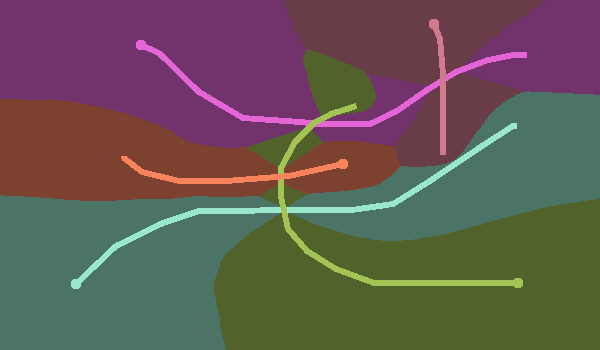
\includegraphics[scale=0.2]{sample004.png} &
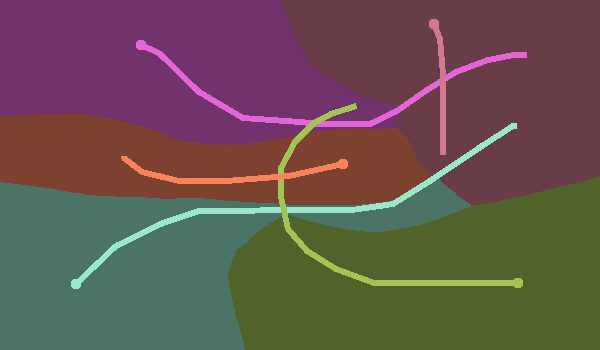
\includegraphics[scale=0.2]{sample020.png} \\
$\nu_{out} / \nu_{in} = 0.04$ & $\nu_{out} / \nu_{in} = 0.20$ \\
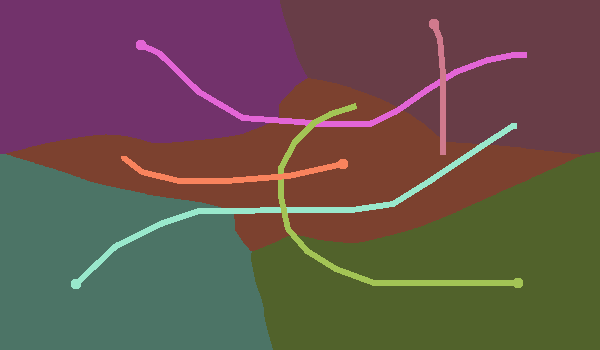
\includegraphics[scale=0.2]{sample050.png} &
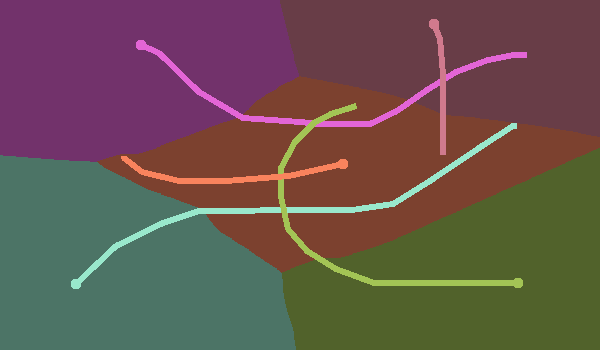
\includegraphics[scale=0.2]{sample080.png} \\
$\nu_{out} / \nu_{in} = 0.50$ & $\nu_{out} / \nu_{in} = 0.80$ \\
\multicolumn{2}{c}{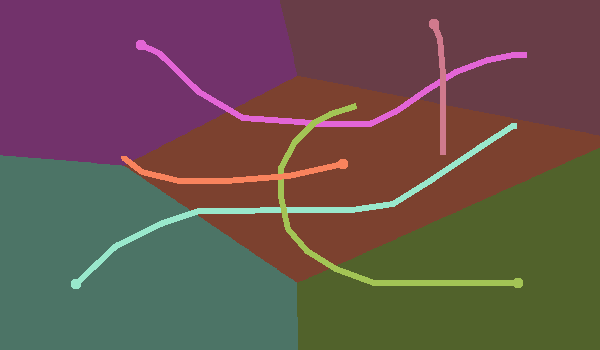
\includegraphics[scale=0.2]{sample100.png}} \\
\multicolumn{2}{c}{$\nu_{out} / \nu_{in} = 1.0$}
\end{tabular}
\end{center}
\caption{Примеры временных диаграмм Вороного, построенные с использованием предложенного метода.}
\label{fig_samples}
\end{figure}

\subsection{Производительность}
Измерения производительности проводились на следующей вычислительной 
конфигурации: центральный процессор --- Intel\textregistered \,
Core\texttrademark \, i7-3610QM CPU, 2.30GHz;
оперативная память --- DDR3 1600 MHz SDRAM, 6144MB; графический процессор 
--- NVidia® GeForce® GTX 660M. Суммарное число отрезков во входных данных
равнялось 100, 1000 и 10000. Так как время работы алгоритма в большей части
зависит от размера текстуры, а не от числа отрезков, то приводятся
результаты тестирования на текстурах со следующим разрешением: 
$1024 \times 1024$, $2048 \times 2048$, $4096 \times 4096$, $8192 \times 8192$. 
Результаты приведены на рис.~\ref{fig_perf}.

\begin{figure}
\begin{center}
\begin{tabular}{l l}
\begin{tikzpicture}
\begin{axis}[
    xtick = {1, 2, 3, 4},
    xticklabels={1024, 2048, 4096, 8192},
    ylabel = время работы (секунды),
    xlabel = $n$ --- размер текстуры (текселей),
    legend style={at={(0.5,1.1)},
        anchor=south,legend columns=3},
    ]
    \addplot+[sharp plot] coordinates
        {(1, 0.070) (2,0.299) (3,1.284) (4,5.470)};
    \addplot+[sharp plot] coordinates
        {(1, 0.078) (2,0.328) (3,1.399) (4,5.956)};
    \addplot+[sharp plot, nodes near coords, 
        style={
           /pgf/number format/fixed,
           /pgf/number format/precision=3,
        }] coordinates {(1, 0.092) (2,0.387) (3,1.616) (4,6.676)};
    \legend{100, 1000, 10000};
\end{axis}
\end{tikzpicture}
&
\begin{tikzpicture}
\begin{axis}[
    xtick = {1, 2, 3, 4},
    xticklabels={1024, 2048, 4096, 8192},
    ylabel = время работы (миллисекунды),
    xlabel = $n$ --- размер текстуры (текселей),
    legend style={at={(0.5,1.1)},
        anchor=south,legend columns=3},
    ]
    \addplot+[sharp plot] coordinates
        {(1, 0.05) (2, 0.08) (3, 0.14) (4,0.26)};
    \addplot+[sharp plot, nodes near coords] coordinates
        {(1, 1.76) (2,3.12) (3, 2.5) (4,2.56)};
    \addplot+[sharp plot, nodes near coords] coordinates
        {(1, 36) (2,38.6) (3,36.7) (4,31)};
    \legend{100, 1000, 10000};
\end{axis}
\end{tikzpicture}
\end{tabular}
\end{center}
\caption{Время работы отдельных частей метода. Справа --- время работы 
итераций \emph{JFA+1}, слева --- время, потраченное на растеризацию.
Различные графики соответствую различному числу отрезков-источников. }
\label{fig_perf}
\end{figure}

\paragraph{Сравнение с предыдущими методами.} Сравнивая приведенные графики 
с графиками, представленными в подразделе \ref{gvd}, можно заметить, что 
новый алгоритм работает приблизительно в три раза медленней, чем алгоритм, описанный
в работе~\cite{gvd}.

\paragraph{Причины потери производительности.} Первое узкое место алгоритма --- это большое число обращений к памяти:
для обработки одного элемента нужно было считать и записать приблизительно 164 байта,
поскольку при разрешении текстуры, равном $n$, число итераций алгоритма составляет
$\mathrm{steps} = \lfloor \log n \rfloor + 1$, то суммарное число считанных/записанных байт 
можно  оценить как $\mathrm{BytesAccessed} = \mathrm{steps} \cdot n^2 \cdot 164$. При этом 
в случае считывании данных об источниках, как уже было замечено ранее, возможно
падение пропускной способности памяти в несколько раз меньше пиковой. Пропускная
способность алгоритма оказалось равной приблизительно 27GB/s, при том что пиковая 
составляет 64GB/s. Заметим, что с увеличением числа источников время выполнения 
\emph{JFA+1} также растет, из чего можно сделать вывод о том, что при небольшом 
числе источников данные о них могут умещаться кэш (объемом 48KB).
Также в этой ситуации, соседние ячейки часто будет ссылаться на одинаковые 
источники, и при обращении к ячейкам данные об этом источнике можно считывать
лишь один раз.

Следующее узкое место алгоритма --- это вычисление оптимального пути от отрезка
до точки, которое заметно сложнее, чем подобные вычисления в работах~\cite{jfa, gvd}.

\subsection{Оценка ошибок}
Для оценки числа ошибок на графическом процессоре был реализован наивный метод
вычисления диаграммы Вороного. Его кратко можно описать следующим образом:
для каждой ячейки перебираются все существующие источники, и наилучший из них записывается 
в ячейку. Оказалось, что для текстуры разрешением $512 \times 512$ относительное 
число ошибок не превышает одного процента и быстро убывает с 
уменьшением шага дискретизации. Полученная точность в целом близка к полученной
в работе~\cite{gvd}.

\section{Дальнейшие исследования}
\label{future}
\paragraph{Улучшение производительности.} На данный момент затруднительно получить
подробную информацию об исполнении шейдеров, и сами вычислительные шейдера ---
относительное недавнее нововведение. Платформа CUDA (унифицированная 
архитектура вычислительных устройств, англ. Compute Unified Device Architechture), 
с другой стороны, обладает богатым набором средств профилирования 
(например NVidia\textregistered Visual Profiler), 
более подробной вычислительной моделью и существует с 2007-ого года. В связи с этим, 
представляется полезным перенести алгоритм на данную архитектуру,
что даст возможность собрать больше информации о его узких местах 
и найти новые пути повышения производительности.

\paragraph{Сплайны.} Было бы интересно ввести источники, задаваемые в виде сплайнов,
которые применяются в картографии и компьютерной графике весьма часто. 
Основную сложность здесь представляет поиск оптимального пути от сегмента 
сплайна до произвольной точки --- аналог метода из подраздела \ref{segopt}.

\paragraph{Многократное использование источников.} В данной работе скорость
источника использовалось только один раз в начале пути.
Как уже было сказано, это достаточно серьезное ограничение, которое не позволит 
получить сколько-нибудь правильные оценки на время от точки до источника
для широкого класса входных данных, которые не подпадают под 
сделанные в данной работе предположения (см. подраздел \ref{props}). Отыскание способа
снять данные ограничение расширит область применимости метода.

\section{Вывод}
Предложенный в данной работе метод решает поставленную задачу (см. раздел \ref{task})
и строит дискретную временную диаграмму Вороного, используя возможности графических
процессоров. При этом число ошибок в построенной диаграмме очень мало по 
сравнению с числом ячеек в дискретизации области. 

Основной проблемой метода оказывается относительно низкая производительность. 
Он работает приблизительно в два раза дольше, чем метод построения обобщенных диаграмм, 
описанный в работе \cite{gvd} (однако там использовалась более профессиональная видеокарта). 
Впрочем, во-первых, есть возможность дальнейшей оптимизации
(см. раздел \ref{future}), а во-вторых, при небольшом разрешении ($512\times512$)
время работы пригодно для использовании при визуализации в режиме
реального времени.

У изначальной постановки задачи существует принципиальный недостаток в том, 
что наличие нескольких областей неоднородности на пути от источника до точки
никак не учитывается, и в общем случае вычисленное время не соответствует 
реальности. Тем не менее для некоторых входных данных этот недостаток несущественен.

В итоге реализованный метод позволяет до некоторой степени верности строить
диаграммы Вороного, основанные на времени, при наличии 
прямолинейных высокоскоростных участков. Используя метод, 
представленный в подразделе~\ref{multi_type}, можно ценой времени работы
алгоритма получить возможность использовать области с различными 
значениями $v_{out}$.
\pagebreak

\begin{appendix}
\section{Исходный код}
\label{source}
Исходный код реализации можно найти по следующей ссылке: 

\url{https://github.com/pschuprikov/cg-miscellaneous/tree/master/time_voronoi_diagrams}.

Исходный код данного отчета можно найти со ссылке:

\url{https://github.com/pschuprikov/psc-itmo-labs/tree/master/shalyto}.

\end{appendix}

\begin{thebibliography}{10}
\bibitem{survey} Franz Aurenhammer. \textit{Voronoi Diagramm --- A Survey of a Fundamental Geomteric Data Structure} 
ACM Computing Surveys, Vol. 23, No. 3, 1991~г.
\bibitem{proced} David S. Elbert et al. \textit{Texturing and Modelling, Third Edition: A Procedural Approach}. 
Morgan Kaufmann, 2002~г.
\bibitem{timeb} D. T. Lee, C. S. Liao, W. B. Wang. \textit{Time-Based Voronoi Diagram}.
\bibitem{cormen} Т. Кормен, Ч. Лейзерсон, Р. Ривест, К. Штайн. \textit{Алгоритмы:
Построение и анализ, Второе издание.} Вильямс, 2010~г.
\bibitem{distmap} Danielsson P. E. \textit{Euclidian Distance Mapping}. Computer Graphics and Image Processing 14, 1980~г.
\bibitem{jfa} Guodong Rong, Tiow-Seng Tan. \textit{Jump Flooding in GPU with Applications to Voronoi Diagram and Distance Transform}. School of Computing, 
National University of Singapore, National University of Singapore, 2006~г. 
\bibitem{gvd} Zhan Yuan, Guodong Rong, Xiaohu Guo, Wenping Wang. \textit{Generalized Voronoi Diagram Computation on GPU}. The University of Hong Kong, The University of Texas at Dallas, 2011~г.
\end{thebibliography}
\end{document}